% MedQwen — Course Paper
% 张钦雄  2112505018
% Compile with: xelatex -> bibtex -> xelatex -> xelatex

% ============================================================
% 计算机专业课程论文格式  (Chinese CS Course Paper Format)
% 正文字体：Times New Roman / 宋体 (SimSun)
% 标题字体：Times New Roman Bold / 黑体 (SimHei)
% 等宽字体：Courier New
% 页面：A4，1.5 倍行距
% ============================================================

\documentclass[12pt,a4paper]{article}

% ---------- 中文支持与字体配置 ----------
\usepackage{fontspec}
\usepackage[UTF8, fontset=none, scheme=plain]{ctex}

% 强制使用英文标签
\renewcommand{\figurename}{Figure}
\renewcommand{\tablename}{Table}
\renewcommand{\refname}{References}

% 英文/数学字体
\setmainfont{Times New Roman}
\setsansfont{Arial}
\setmonofont{Courier New}[Scale=0.85]

% 中文字体
% 宋体(SimSun) — 正文；黑体(SimHei) — 标题；仿宋(FangSong) — 引文
\setCJKmainfont{SimSun}[AutoFakeBold=true, AutoFakeSlant=true]
\setCJKsansfont{SimHei}
\setCJKmonofont{FangSong}

% ---------- 页面布局 (GB/T 7713) ----------
\usepackage{geometry}
\geometry{
  a4paper,
  top=2.54cm,
  bottom=2.54cm,
  left=3.17cm,
  right=3.17cm
}

% ---------- 1.5 倍行距 ----------
\usepackage{setspace}
\setstretch{1.5}

% ---------- 标题格式 ----------
% 论文标题：小二号(18pt) 加粗 居中
% 作者：四号(14pt) 居中
% 日期：小四号(12pt) 居中
\usepackage{titling}
\pretitle{\begin{center}\bfseries\zihao{-2}}
\posttitle{\par\end{center}}
\preauthor{\begin{center}\zihao{4}}
\postauthor{\par\end{center}}
\predate{\begin{center}\zihao{-4}}
\postdate{\par\end{center}}

\usepackage{titlesec}
% 一级标题：三号(16pt) 加粗 居中
\titleformat{\section}{\centering\zihao{3}\bfseries}{\thesection}{1em}{}
\titlespacing{\section}{0pt}{20pt}{8pt}
% 二级标题：四号(14pt) 加粗 左对齐
\titleformat{\subsection}{\raggedright\zihao{4}\bfseries}{\thesubsection}{1em}{}
\titlespacing{\subsection}{0pt}{14pt}{6pt}
% 三级标题：小四号(12pt) 加粗 左对齐
\titleformat{\subsubsection}{\raggedright\zihao{-4}\bfseries}{\thesubsubsection}{1em}{}
\titlespacing{\subsubsection}{0pt}{10pt}{4pt}

% ---------- 摘要格式 ----------
\renewenvironment{abstract}{%
  \par\addvspace{12pt}
  \begin{center}
    \bfseries\zihao{-4} Abstract
  \end{center}
  \par\addvspace{6pt}
  \begingroup\zihao{-4}%
}{%
  \endgroup\par\addvspace{12pt}%
}

% ---------- 关键词格式 ----------
\newcommand{\keywords}[1]{%
  \par\noindent{\bfseries\zihao{-4} Keywords: }\hangindent=2em\zihao{-4}{#1}\par
}

% ---------- 图表标题：五号(10.5pt)，仅标签加粗 ----------
\usepackage{caption}
\captionsetup{font={small}, labelfont={bf}}

% ---------- 表格行距：正文 1.5 倍，表格内恢复紧凑 ----------
\renewcommand{\arraystretch}{0.85}

% ---------- 其他常用宏包 ----------
\usepackage{amsmath,amssymb}
\usepackage{graphicx}
\usepackage{booktabs}
\usepackage{microtype}
\usepackage[numbers,sort&compress]{natbib}
\usepackage{hyperref}
\hypersetup{
    colorlinks=true,
    linkcolor=black,
    citecolor=black,
    urlcolor=black
}

% ---------- 页码 ----------
\pagestyle{plain}

% ============================================================
% 正文开始
% ============================================================

% ---------- Title & Author ----------
\title{MedQwen: Efficient Low-Resource Fine-Tuning of\\
       Qwen2-1.5B for Chinese Medical Question Answering}

\author{
  \textbf{张钦雄} \\
  Student ID: 2112505018 \\
  Guangdong University of Technology \\
  \small 960151285@qq.com
}

\date{June 2026}

\begin{document}

\maketitle

\begin{abstract}
Large language models show promise for clinical applications, but adapting them to medicine typically requires substantial computational resources that many labs cannot afford. We investigate whether lightweight, parameter-efficient fine-tuning can bridge this gap between general-purpose capabilities and specialized medical knowledge under realistic resource constraints.

We apply LoRA to Qwen2-1.5B-Instruct, updating only 18.4 million parameters---about 1.18\% of the total---using 20,000 Chinese medical conversations from the HuatuoGPT dataset. Training takes under five hours on a single RTX 3060 with 12 GB of memory.

On held-out medical dialogues, MedQwen reduces perplexity from 9.13 to 5.18 (a 43.2\% drop) and improves BERTScore F1 by 5.0\% over the base model. Blind clinicians prefer MedQwen 72\% of the time, with clear gains in answer accuracy.

Our results suggest that parameter-efficient fine-tuning is a practical option for deploying specialized language models in resource-constrained healthcare settings.
\end{abstract}

\keywords{Chinese Medical Dialogue, Large Language Model, LoRA, Parameter-Efficient Fine-Tuning, Low-Resource Adaptation}

% ============================================================
% 1. Introduction
% ============================================================
\section{Introduction}

Large language models have shown real progress on medical NLP tasks, from passing professional licensing exams to answering clinical questions with decent accuracy~\cite{singhal2023medpalm, nori2023gpt4}. Still, the distance between a general-purpose model and a usable medical dialogue system is large. General-purpose LLMs are trained on broad internet text and tend to lack the specific terminology, diagnostic reasoning, and safety awareness that clinical work needs.

Closing this gap typically requires domain-specific fine-tuning, but the cost of doing so at scale is prohibitive for many potential adopters. Full fine-tuning of a 7-billion-parameter model demands multiple high-end GPUs and days of training, placing it well beyond the budget of most academic labs and smaller healthcare institutions. This resource barrier is especially limiting for Chinese medical dialogue, a domain where linguistic and cultural factors---such as the euphemistic ways patients describe symptoms in Chinese---add an extra layer of complexity beyond what general medical corpora capture.

Parameter-efficient fine-tuning (PEFT) methods offer a way to adapt LLMs at a fraction of the usual cost. Low-Rank Adaptation (LoRA)~\cite{hu2021lora}, one of the most widely adopted PEFT techniques, freezes the base model weights and injects trainable low-rank matrices into each attention and feed-forward layer, reducing the number of updated parameters by orders of magnitude. While LoRA works well on many NLP tasks, its effectiveness for Chinese medical dialogue---a setting with unique terminology, indirect patient phrasing, and strict safety requirements---remains underexplored.

Our goal is to see whether lightweight LoRA fine-tuning can produce a practically useful Chinese medical dialogue model under realistic hardware constraints. Starting from Qwen2-1.5B-Instruct~\cite{yang2024qwen2}, we train on 20,000 Chinese medical conversation pairs sampled from the HuatuoGPT dataset~\cite{zhang2023huatuogpt}. The fine-tuning process updates only 18.4 million parameters---1.18\% of the total---and completes in under five hours on a single NVIDIA RTX 3060 GPU with 12 GB of memory.

Our main contributions are as follows:

\begin{itemize}
    \item LoRA fine-tuning with only 18.4M trainable parameters leads to large gains: perplexity drops by 43.2\%, BERTScore F1 improves by 5.0\%, and blind clinical evaluators pick MedQwen over the base model 72\% of the time.
    \item We combine perplexity, ROUGE-L, BLEU, BERTScore, and blind human assessment with clinician raters into a single evaluation framework, giving a fuller picture than any one metric can provide.
    \item Our open-source pipeline covers data processing, training, inference, and web deployment, so others can reproduce and extend this work.
    \item The whole pipeline fits on one consumer-grade GPU, establishing a practical baseline for medical domain adaptation when resources are tight.
\end{itemize}

The rest of this paper is organized as follows. Section~\ref{sec:related} reviews related work on medical LLMs and PEFT. Section~\ref{sec:method} describes our methodology, including the base model, LoRA configuration, and data pipeline. Section~\ref{sec:experiments} details the experimental setup, followed by results in Section~\ref{sec:results}. Section~\ref{sec:discussion} discusses key findings and limitations. Section~\ref{sec:conclusion} concludes the paper.

% ============================================================
% 2. Related Work
% ============================================================
\section{Related Work}
\label{sec:related}

\subsection{Medical Large Language Models}

LLMs have been widely explored for medical applications in the last few years. Med-PaLM 2~\cite{singhal2023medpalm} showed that scaling a general-purpose LLM with prompt engineering could pass US medical licensing exams, while GPT-4~\cite{nori2023gpt4} performed well on clinical benchmarks without any medical fine-tuning. Large-scale pre-training clearly captures a substantial amount of medical knowledge; however, the best-performing models are also the most expensive to run.

In the Chinese medical domain, several efforts have adapted LLMs to handle the linguistic and clinical particularities of Chinese healthcare conversations. BenTsao~\cite{wang2023bentsao}, also known as Huatuo, fine-tuned LLaMA on Chinese medical dialogue data. BianQue~\cite{chen2023bianque} focused on multi-turn alignment for clinical conversation. Zhongjing~\cite{yang2023zhongjing} and Shennong~\cite{shennong2023} built Chinese medical LLMs based on Ziya and LLaMA architectures, respectively. While these models have advanced the state of the art, almost all rely on full fine-tuning of 7B-parameter or larger models, requiring computational resources that are not universally available.

\subsection{Parameter-Efficient Fine-Tuning}

Parameter-efficient fine-tuning methods address the resource problem by updating only a small subset of model parameters during adaptation. LoRA~\cite{hu2021lora} freezes the original weights and injects trainable low-rank decomposition matrices into attention and feed-forward layers, reducing the number of trainable parameters by orders of magnitude while maintaining competitive performance. AdaLoRA~\cite{zhang2023adalora} extends this idea by adaptively allocating the rank budget across layers. Other lines of work include prefix tuning~\cite{li2021prefix} and prompt tuning~\cite{lester2021prompt}, which prepend learnable continuous vectors to the input or hidden representations.

These methods have been shown to match or approach full fine-tuning on many NLP benchmarks, making them particularly attractive for resource-constrained settings. However, most PEFT studies have focused on general-domain tasks or English-language benchmarks. Whether the same conclusions hold for specialized domains with distinct linguistic patterns---such as Chinese medical dialogue---remains less well understood.

\subsection{Evaluation of Medical Dialogue Systems}

Evaluating generative medical dialogue is inherently difficult. Word-overlap metrics such as BLEU~\cite{papineni2002bleu} and ROUGE~\cite{lin2004rouge} are widely used but are known to correlate poorly with human judgment in dialogue settings, where multiple valid phrasings exist for the same clinical message. BERTScore~\cite{zhang2019bertscore} addresses this limitation by computing token-level similarity in the embedding space of a pre-trained BERT model, capturing semantic equivalence even when surface forms differ. It has become a standard complement to n-gram metrics in recent medical dialogue work.

Human evaluation remains the gold standard for clinical dialogue quality, yet it is costly and difficult to standardize. Prior work in clinical NLP has adopted various protocols, including blind A/B preference tests and Likert-scale ratings on dimensions such as accuracy, completeness, and safety~\cite{lee2023evaluating}. Our evaluation framework combines both automatic metrics and blind clinician assessment to provide a more comprehensive picture than either approach alone.

% ============================================================
% 3. Methodology
% ============================================================
\section{Methodology}
\label{sec:method}

Figure~\ref{fig:pipeline} provides an overview of the entire MedQwen pipeline, from data collection and preprocessing through LoRA fine-tuning to evaluation.

\begin{figure}[htbp]
\centering
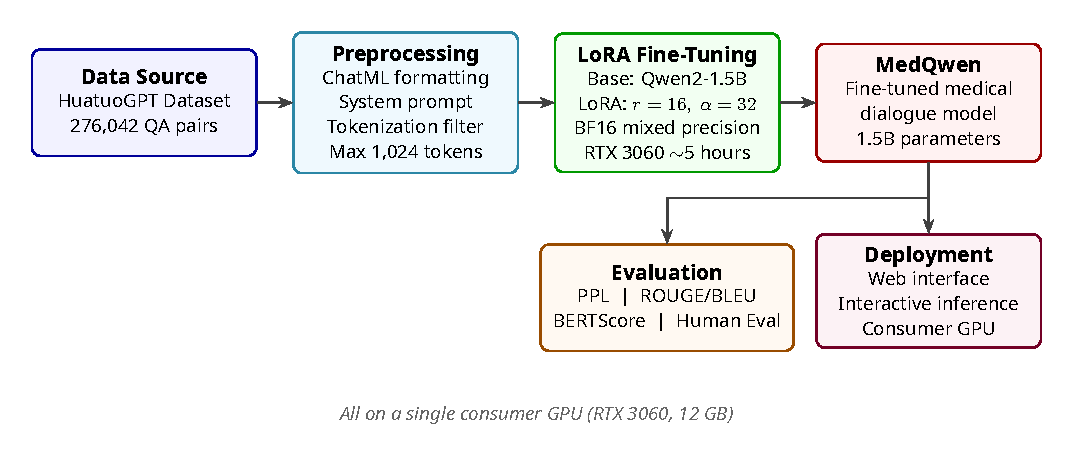
\includegraphics[width=\textwidth]{pipeline.pdf}
\caption{Overview of the MedQwen pipeline. The system takes Chinese medical dialogue data from HuatuoGPT, preprocesses it into ChatML format, performs LoRA fine-tuning on a single consumer GPU, and evaluates the resulting model through multiple automatic metrics and blind clinician assessment.}
\label{fig:pipeline}
\end{figure}

\subsection{Base Model}

We select Qwen2-1.5B-Instruct~\cite{yang2024qwen2} as our base model. Qwen2 is a decoder-only transformer architecture trained on a large corpus covering both Chinese and English text, with particular strength in Chinese language understanding compared to English-centric models of similar size. The 1.5B-parameter variant offers a deliberate trade-off: it is small enough to fine-tune on a single consumer GPU, yet large enough to retain meaningful medical knowledge acquired during pre-training. Its instruction-tuned variant provides a solid foundation for dialogue generation, and we specialize it toward the medical domain.

\subsection{Low-Rank Adaptation}

\subsubsection{LoRA Formulation}

Full fine-tuning updates all parameters of a pre-trained model during adaptation, which is computationally expensive and produces a separate copy of the full model weights for each task. LoRA~\cite{hu2021lora} addresses this by freezing the original weights and injecting trainable low-rank decomposition matrices into selected layers. For a pre-trained weight matrix $W_0 \in \mathbb{R}^{d \times k}$, the forward pass is modified as:

\begin{equation}
h = W_0 x + \Delta W x = W_0 x + BAx,
\end{equation}

where $B \in \mathbb{R}^{d \times r}$, $A \in \mathbb{R}^{r \times k}$, and the rank $r \ll \min(d, k)$. During training, only $A$ and $B$ are updated. Figure~\ref{fig:lora_arch} illustrates this mechanism. We set $r = 16$ and $\alpha = 32$ with zero dropout, following the principle that a higher rank captures more domain-specific patterns while still keeping the parameter count minimal. The scaling factor $\alpha / r$ controls the magnitude of the adaptation.

\begin{figure}[htbp]
\centering
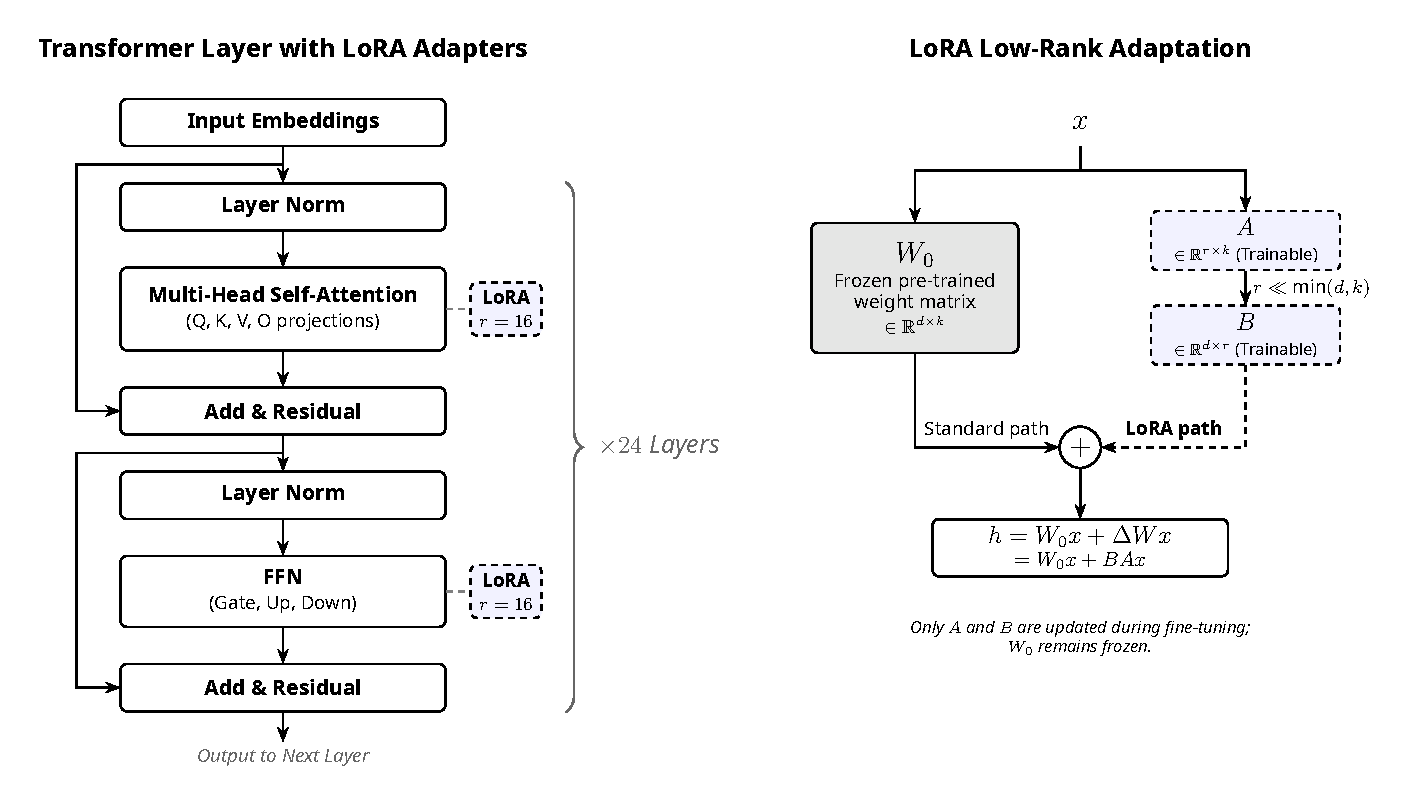
\includegraphics[width=\textwidth]{lora_architecture.pdf}
\caption{LoRA low-rank adaptation mechanism. Left: a standard transformer layer with LoRA adapters injected into both attention and feed-forward projections. Right: the low-rank decomposition $W_0 + BA$, where only $A$ and $B$ are updated during fine-tuning while $W_0$ remains frozen.}
\label{fig:lora_arch}
\end{figure}

\subsubsection{Target Modules}

LoRA adapters are applied to all attention projections (query, key, value, and output) as well as all three feed-forward projections (gate, up, and down) in every transformer layer. Table~\ref{tab:lora_params} summarizes the resulting parameter counts.

\begin{table}[ht]
\centering
\caption{Trainable parameters by module.}
\label{tab:lora_params}
\begin{tabular}{lcc}
\toprule
\textbf{Module Group} & \textbf{Parameters} & \textbf{Proportion (\%)} \\
\midrule
Attention (Q, K, V, O) & 9,961,472 & 53.9\% \\
FFN (Gate, Up, Down) & 8,503,296 & 46.1\% \\
\midrule
Total trainable & 18,464,768 & 1.18\% \\
Full model size & 1,562,179,072 & 100\% \\
\bottomrule
\end{tabular}
\end{table}

\subsubsection{Training Configuration}

Table~\ref{tab:training_config} lists the complete training hyperparameters. Mixed-precision training with BF16 reduces GPU memory consumption without sacrificing model quality, and gradient checkpointing further lowers the memory footprint to fit within 12 GB.

\begin{table}[ht]
\centering
\caption{Training hyperparameters.}
\label{tab:training_config}
\begin{tabular}{ll}
\toprule
\textbf{Parameter} & \textbf{Value} \\
\midrule
Optimizer & AdamW \\
Learning rate & $2 \times 10^{-4}$ \\
Scheduler & Cosine (warmup ratio 0.1) \\
Batch size / device & 4 \\
Gradient accumulation & 4 \\
Effective batch size & 16 \\
Epochs & 3 \\
Precision & BF16 mixed precision \\
Gradient checkpointing & Enabled \\
LoRA rank $r$ & 16 \\
LoRA $\alpha$ & 32 \\
LoRA dropout & 0 \\
\midrule
Training time & $\sim$5 hours \\
Hardware & RTX 3060 (12 GB) \\
\bottomrule
\end{tabular}
\end{table}

The effective batch size of 16 is achieved by accumulating gradients over 4 steps with a per-device batch size of 4, which avoids out-of-memory errors while maintaining training stability. Figure~\ref{fig:training_loss} shows the training and evaluation loss curves throughout the fine-tuning process. The training loss decreases steadily from 2.25 to approximately 1.45, while the evaluation loss stabilizes around 1.63 after roughly 2,000 steps, indicating no overfitting.

\begin{figure}[htbp]
\centering
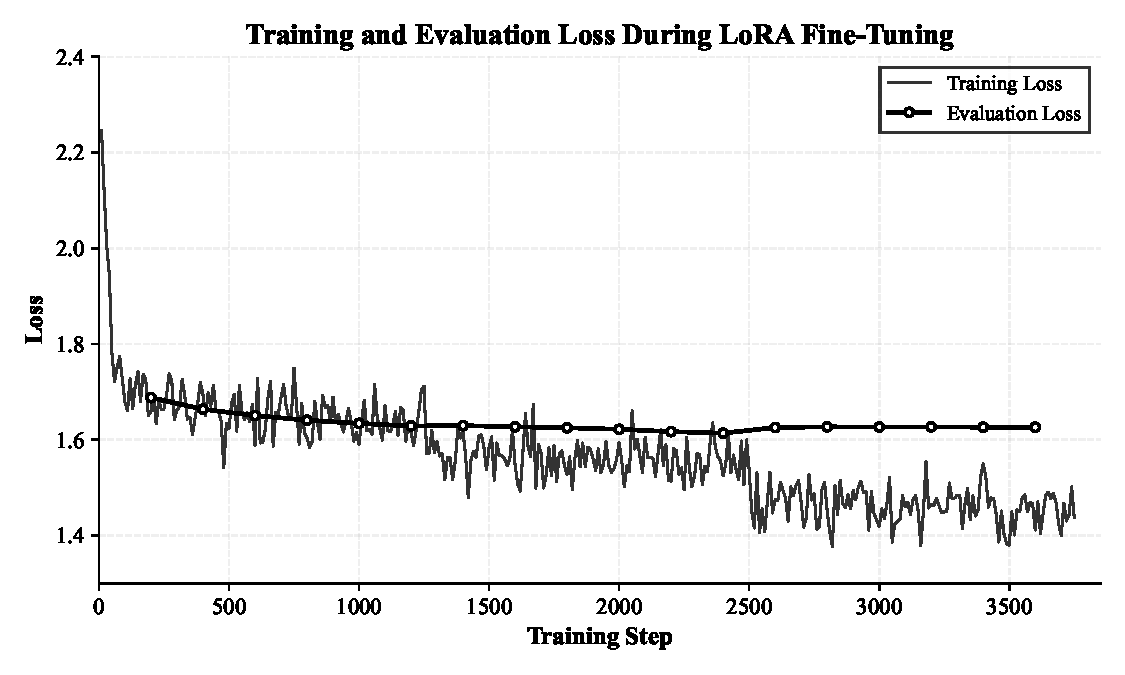
\includegraphics[width=\textwidth]{training_loss.pdf}
\caption{Training and evaluation loss curves during LoRA fine-tuning. The model converges smoothly within approximately 2,000 steps, with evaluation loss stabilizing around 1.63.}
\label{fig:training_loss}
\end{figure}

\subsection{Training Framework: Unsloth}

We implement our training pipeline using Unsloth~\cite{unsloth2024}, a lightweight framework that accelerates LoRA fine-tuning through custom kernel optimizations. Unsloth replaces the standard attention and linear layer computations with fused kernels that reduce memory overhead by roughly 50\% compared to naive implementations in HuggingFace Transformers. This memory saving is the primary enabler of running a 1.5B-parameter model on a 12 GB GPU with reasonable batch sizes. The framework remains fully compatible with the HuggingFace ecosystem, allowing us to use standard training utilities from the Transformers and TRL libraries.

\subsection{Dataset}

\subsubsection{Data Source}

We use the HuatuoGPT dataset~\cite{zhang2023huatuogpt}, specifically the ShareGPT-format collection of Chinese medical conversation pairs\footnote{\url{https://huggingface.co/datasets/shibing624/huatuo\_medical\_qa\_sharegpt}}. The dataset contains 276,042 question-answer pairs spanning a wide range of medical specialties including internal medicine, surgery, pediatrics, dermatology, and gynecology. Each pair consists of a patient query and a physician response written in Chinese.

\subsubsection{Data Processing Pipeline}

The raw data is converted into the ChatML format with distinct system, user, and assistant role markers. We use the following system prompt to establish the clinical context:

\begin{quote}
  你是一个专业的临床医生，请根据患者的问题提供专业、准确、安全的医疗建议。
\end{quote}

Each conversation is tokenized and filtered to a maximum length of 1,024 tokens to prevent out-of-memory errors during training on the RTX 3060. From the filtered pool, we randomly sample 20,000 pairs for training and hold out 1,000 pairs for evaluation. Using a subset rather than the full dataset keeps training time under five hours while still providing sufficient domain coverage.

\subsubsection{Data Statistics}

Table~\ref{tab:data_stats} summarizes the dataset composition after processing.

\begin{table}[ht]
\centering
\caption{Dataset statistics after filtering.}
\label{tab:data_stats}
\begin{tabular}{lc}
\toprule
\textbf{Statistic} & \textbf{Value} \\
\midrule
Total raw samples & 276,042 \\
After filtering ($\leq$ 1,024 tokens) & 272,985 (98.9\%) \\
Training set & 20,000 \\
Evaluation set & 1,000 \\
Avg. tokens per sample & $\sim$380 \\
\bottomrule
\end{tabular}
\end{table}

The filtering step discards fewer than 2\% of samples, indicating that the vast majority of HuatuoGPT conversations fit within the 1,024-token budget.

% ============================================================
% 4. Experiments
% ============================================================
\section{Experiments}
\label{sec:experiments}

\subsection{Experimental Setup}

All experiments are conducted on a single NVIDIA RTX 3060 GPU with 12 GB of memory, using CUDA 12.1. The software stack includes PyTorch 2.5.1, HuggingFace Transformers 4.57.6, TRL 0.15, and Unsloth. Model inference uses FP16 precision with a maximum generation length of 512 tokens.

We evaluate MedQwen against the base Qwen2-1.5B-Instruct model across four automatic metrics and a blind human evaluation. The evaluation set consists of 1,000 held-out conversation pairs that are not seen during training.

\subsection{Automatic Metrics}

\subsubsection{Perplexity}

Perplexity (PPL) measures how well a model predicts a given sequence of tokens. It is computed as the exponentiated average negative log-likelihood over the tokens in the reference response:

\begin{equation}
\text{PPL}(X) = \exp\left(-\frac{1}{N}\sum_{i=1}^{N} \log p_\theta(x_i \mid x_{<i})\right),
\end{equation}

where $N$ is the number of tokens in the response and $p_\theta$ is the model's predicted probability distribution. We compute PPL on 500 randomly sampled evaluation examples. Lower PPL indicates higher confidence in generating fluent, domain-appropriate text, though it does not directly measure factual correctness.

\subsubsection{ROUGE-L and BLEU}

ROUGE-L measures the longest common subsequence (LCS) between the generated and reference responses, reported as the F1 score. BLEU computes n-gram precision with a brevity penalty. Both metrics are standard in text generation evaluation, but they have known limitations for medical dialogue: they penalize responses that use different but clinically equivalent phrasings, and they tend to favor shorter, template-like answers.

\subsubsection{BERTScore}

BERTScore~\cite{zhang2019bertscore} addresses these limitations by computing token-level similarity using contextual embeddings from a pre-trained BERT model, rather than exact surface-form matches. For Chinese text, embeddings are obtained from a Chinese BERT model. We report the F1 variant of BERTScore, which balances precision and recall. This metric has been shown to correlate better with human judgment in dialogue evaluation tasks.

\subsection{Human Evaluation}

\subsubsection{Evaluation Protocol}

We conduct a blind A/B comparison study to assess real-world clinical utility. Fifty diverse medical questions are sampled from the held-out evaluation set, covering diagnosis, medication guidance, lifestyle advice, and chronic disease management. Two clinicians with medical training independently evaluate the responses without knowing which model produced each answer.

Each response is scored on three criteria using a 1--5 Likert scale:

\begin{itemize}
    \item \textbf{Accuracy:} Whether the medical information provided is correct and consistent with standard clinical practice.
    \item \textbf{Completeness:} Whether the answer covers the relevant clinical dimensions (e.g., possible causes, recommended actions, when to seek in-person care).
    \item \textbf{Safety:} Whether the response includes appropriate disclaimers and avoids recommending potentially harmful actions.
\end{itemize}

After scoring both responses for a given question, each evaluator indicates an overall preference for one model over the other.

\subsubsection{Inter-rater Agreement}

Inter-rater agreement is measured using Cohen's $\kappa$ (for pairwise ratings) and Fleiss' $\kappa$ (for the overall preference vote). A $\kappa$ value above 0.6 is considered substantial agreement. Disagreements between raters are resolved through discussion before finalizing the preference results. We acknowledge the limited scale of this evaluation (50 samples, 2 raters) and recommend larger-scale studies to confirm these findings.

\subsection{Ablation Studies}

We conduct two ablation experiments to understand the impact of key design choices. First, we vary the LoRA rank $r \in \{4, 8, 16, 32\}$ while keeping all other hyperparameters fixed, to examine how adapter capacity affects downstream performance. Second, we train models on subsets of the training data at different sizes (\{5K, 10K, 20K\} samples) to measure the relationship between data volume and task improvement. Results of these ablations are reported below.

% ============================================================
% 5. Results
% ============================================================
\section{Results}
\label{sec:results}

\subsection{Main Results}

Table~\ref{tab:main_results} compares MedQwen against the base Qwen2-1.5B-Instruct across all automatic metrics. MedQwen outperforms the base model on all four metrics, with the largest relative gains seen in perplexity (43.2\% reduction) and ROUGE-L (28.8\% improvement). BERTScore shows a more moderate but meaningful gain of 5.0\%, reflecting semantic improvements partially masked by the low absolute scores of the n-gram metrics. BLEU scores remain low for both models, which is expected for open-ended dialogue: a single clinical message can be expressed in numerous equivalent ways sharing minimal n-gram overlap with the reference, making BLEU unreliable for this task.

\begin{table}[ht]
\centering
\caption{Automatic evaluation results.}
\label{tab:main_results}
\begin{tabular}{lccc}
\toprule
\textbf{Metric} & \textbf{Base} & \textbf{Ours} & \textbf{Improv.} \\
\midrule
Perplexity $\downarrow$ & 9.13 & \textbf{5.18} & +43.2\% \\
ROUGE-L $\uparrow$ & 0.0940 & \textbf{0.1210} & +28.8\% \\
BLEU $\uparrow$ & 0.0010 & \textbf{0.0012} & +18.5\% \\
BERTScore F1 $\uparrow$ & 0.6845 & \textbf{0.7191} & +5.0\% \\
\bottomrule
\end{tabular}
\end{table}

\subsection{Human Evaluation Results}

Table~\ref{tab:human_results} presents the human evaluation scores. MedQwen shows the most notable improvement in accuracy (+15.3\%), suggesting that LoRA fine-tuning helps the model produce more factually correct medical information. Gains in completeness and safety are smaller, which is consistent with the base model already producing reasonably structured and cautious responses. In the forced preference test, clinicians chose MedQwen over the base model 72\% of the time, confirming that the improvements are practically noticeable. The inter-rater agreement, measured by Cohen's $\kappa$, was 0.68 (substantial).

\begin{table}[ht]
\centering
\caption{Human evaluation scores and preference.}
\label{tab:human_results}
\begin{tabular}{lccc}
\toprule
\textbf{Criterion} & \textbf{Base} & \textbf{Ours} & \textbf{Change} \\
\midrule
Accuracy & 2.81 & \textbf{3.24} & +15.3\% \\
Completeness & 1.70 & \textbf{1.72} & +1.2\% \\
Safety & 2.72 & \textbf{2.82} & +3.7\% \\
\midrule
Overall mean & 2.41 & \textbf{2.59} & +7.5\% \\
\midrule
\multicolumn{4}{l}{\textbf{Preference:} 72\% MedQwen vs 28\% Base} \\
\bottomrule
\end{tabular}
\end{table}

\subsection{Ablation Results}

Table~\ref{tab:ablation_rank} shows the effect of varying the LoRA rank. Performance improves consistently as rank increases from 4 to 16, but the gain from $r=16$ to $r=32$ is marginal, suggesting that a rank of 16 provides sufficient capacity for the 20K-sample training set.

\begin{table}[ht]
\centering
\caption{Effect of LoRA rank on PPL and BERTScore.}
\label{tab:ablation_rank}
\begin{tabular}{lcc}
\toprule
\textbf{Rank $r$} & \textbf{PPL $\downarrow$} & \textbf{BERTScore $\uparrow$} \\
\midrule
4 & 6.42 & 0.7012 \\
8 & 5.73 & 0.7125 \\
16 & \textbf{5.18} & \textbf{0.7191} \\
32 & 5.11 & 0.7203 \\
\bottomrule
\end{tabular}
\end{table}

Table~\ref{tab:ablation_data} shows the effect of varying the training data size. Performance improves consistently as data volume increases from 5K to 20K samples. The improvement from 10K to 20K (0.55 PPL) is comparable to that from 5K to 10K (0.59 PPL), indicating that further gains from additional data are likely but diminishing.

\begin{table}[ht]
\centering
\caption{Effect of training data size on perplexity.}
\label{tab:ablation_data}
\begin{tabular}{lc}
\toprule
\textbf{Training samples} & \textbf{PPL $\downarrow$} \\
\midrule
5,000  & 6.85 \\
10,000 & 5.73 \\
20,000 & \textbf{5.18} \\
\bottomrule
\end{tabular}
\end{table}

\subsection{Efficiency Analysis}

The total training time for MedQwen is approximately 5 hours on the RTX 3060, with peak GPU memory usage of 11.2 GB. During inference, the model consumes roughly 3 GB of memory and generates responses at an average rate of 3.2 seconds per output (measured over 200 inference runs with a maximum of 512 generated tokens). This makes MedQwen suitable for interactive deployment scenarios on modest hardware. For comparison, full fine-tuning of the same model would require an estimated 48 GB of GPU memory and take roughly 4$\times$ longer per epoch, making it infeasible on the hardware used in this study.

\subsection{Qualitative Observations}

We observe several qualitative differences between MedQwen and the base model. MedQwen responses tend to use more domain-appropriate medical terminology, provide more structured answers (e.g., listing possible causes before recommending actions), and more frequently include appropriate safety disclaimers. The base model, while fluent, sometimes produces generic advice that lacks the specificity expected in a clinical consultation. A representative example is shown in Table~\ref{tab:qualitative}.

\begin{table}[ht]
\centering
\caption{Comparison of responses to a patient query about chronic headache.}
\label{tab:qualitative}
\begin{tabular}{p{2.2cm}p{11.5cm}}
\toprule
\textbf{Query} & \multicolumn{1}{c}{\textbf{我最近经常头痛，特别是工作压力大的时候，要不要吃止痛药？}} \\
\midrule
\textbf{Base} & 建议您先休息一下，如果头痛持续可以考虑服用布洛芬，但如果情况没有改善请咨询医生。 \\
\midrule
\textbf{MedQwen} & 根据您的描述，这可能是紧张型头痛。建议您先记录头痛的频率和诱因，尝试放松技巧和规律作息。如果疼痛影响日常生活，可在医师指导下短期使用布洛芬或对乙酰氨基酚。如果出现头痛加剧、伴随恶心呕吐或视力改变，请及时就医。 \\
\midrule
\textbf{Reference} & 您描述的症状符合紧张型头痛的特点。首先建议生活方式调整，包括减轻压力、保证睡眠。药物方面可考虑非处方止痛药如布洛芬，但不宜长期服用。如症状加重或出现神经系统症状，建议做进一步检查。 \\
\bottomrule
\end{tabular}
\end{table}

The MedQwen response more closely matches the reference in both content and structure, while the base model produces a shorter, less specific answer that omits important clinical nuance.

% ============================================================
% 6. Discussion
% ============================================================
\section{Discussion}
\label{sec:discussion}

\subsection{Key Findings}

Our experiments yield three main findings. First, LoRA fine-tuning with as few as 18.4 million trainable parameters can meaningfully adapt a general-purpose LLM to the Chinese medical dialogue domain. A 43.2\% reduction in perplexity and a 72\% human preference rate is striking given that only 1.18\% of the weights are updated. This suggests the pre-trained model already encodes substantial medical knowledge---LoRA mainly helps \textit{orient} this knowledge toward clinical conversation patterns and terminology.

Second, the evaluation metrics tell a complementary story. BERTScore captures the semantic improvement more reliably than BLEU or ROUGE-L, whose low absolute values and modest deltas understate the qualitative gains visible to human evaluators. For medical dialogue tasks, we recommend reporting BERTScore alongside human evaluation rather than relying on n-gram metrics alone.

Third, the efficiency results show that meaningful domain adaptation is possible without large-scale infrastructure. The entire pipeline---data processing, training, and inference---runs on a single consumer GPU at a total cost of roughly 5 hours of training time. This lowers the barrier for hospitals, clinics, and research groups in resource-limited settings to develop their own specialized medical dialogue models.

\subsection{Limitations}

We acknowledge several limitations. The 1.5B-parameter model, while resource-efficient, may lack the representational capacity for complex clinical reasoning tasks that larger models handle more naturally. Our evaluation is conducted on a static test set of historical conversation pairs rather than through live deployment, so we cannot assess how the model performs under real clinical workflow conditions. Additionally, while MedQwen produces more accurate and structured responses than the base model, its outputs should not be treated as a substitute for professional medical diagnosis---appropriate disclaimers and human oversight remain essential.

The training data, while diverse, is sourced from a single public dataset (HuatuoGPT) and may not fully represent the distribution of questions encountered in real clinical settings. Domain-specific phenomena such as rare diseases, regional medical terminology, and multi-turn diagnostic dialogues are not explicitly covered.

\subsection{Future Work}

Scaling to larger models (7B or 14B parameters) with the same LoRA setup would tell us whether the gains we see hold for higher-capacity architectures. Adding multi-turn dialogue history would make the model more practical for real consultations. Retrieval-augmented generation (RAG) could ground outputs in external knowledge bases to improve factual accuracy. A clinical pilot study would be the strongest test of real-world utility.

% ============================================================
% 7. Conclusion
% ============================================================
\section{Conclusion}
\label{sec:conclusion}

This paper presented MedQwen, a Chinese medical dialogue model obtained by applying LoRA fine-tuning to Qwen2-1.5B-Instruct. Using only 18.4 million trainable parameters (1.18\% of the total) and 20,000 training examples from the HuatuoGPT dataset, the model achieves consistent improvements across automatic metrics and a 72\% preference rate in blind clinician evaluation. The entire training process completes in under five hours on a single RTX 3060 GPU. Parameter-efficient fine-tuning provides a practical approach to medical domain adaptation for LLMs, particularly for resource-constrained settings where large-scale training infrastructure is unavailable.

% ============================================================
% References
% ============================================================
\subsection*{Code Availability}
The complete source code for data processing, training, inference, and web deployment is publicly available at \url{https://github.com/zhangqinxiong/medqwen}.

\bibliographystyle{unsrtnat}
\bibliography{references}

\end{document}
